\section{Introduction}
\subsection{Overview of High-Frequency Trading and Reinforcement Learning}
High-frequency trading (HFT) represents one of the most technologically demanding domains within quantitative finance,
characterized by its need for ultra-low latency, massive volumes of data, and the ability to adapt dynamically to rapidly changing market conditions. 
Reinforcement learning (RL) has emerged as a promising approach for developing trading strategies, 
offering the ability to learn optimal policies directly from market interactions without requiring explicit rules or models.
However, applying RL to HFT is fraught with challenges, particularly when scaling training and inference to meet the performance 
requirements of live trading environments.

Traditional RL frameworks often rely on centralized architectures, where a single learner aggregates experiences from multiple actors to update a shared policy. 
While effective in general-purpose applications, such approaches can become bottlenecks in HFT contexts, 
where the scale and complexity of trading environments demand distributed efficiency and continuous adaptability. 
Moreover, typical RL systems treat environments as isolated entities for each agent or strategy, 
leading to significant computational redundancies when simulating complex environments like the limit order book (LOB).

\subsection{Motivation and Contributions}

This thesis proposes a novel parallel, agent-based RL framework designed specifically for the HFT domain. 
The framework leverages Ray RLlib to parallelize environments and adopts a structure inspired by the actor-learner model introduced in the 
IMPALA (Importance Weighted Actor-Learner Architecture) algorithm. 
However, it extends this paradigm by introducing multiple learners, each corresponding to a unique agent definition, 
and enabling workers from different learners to share the same distributed LOB environment. 
This design reduces computational overhead by reusing core environment components, such as order aggregation, order book initialization,
and transaction processing, across multiple agents.

The primary contributions of this thesis are as follows:

\begin{itemize}
  \item A Parallel Agent-Based Framework: A system architecture enabling the efficient deployment, configuration, and adaptation of individual RL agents, 
    each capable of distributed training and leveraging shared environments.

  \item Shared Limit Order Book Environments: An innovative mechanism for reducing redundant computations by allowing multiple workers, 
    assigned to different learners, to interact with a shared, distributed LOB environment.

  \item Continuous Training and Deployment Pipeline: A framework supporting the dynamic training and deployment of multiple strategies, 
    enabling real-time adaptation to changing market conditions—a critical requirement in HFT.
\end{itemize}


The framework must scale effectively with the number of agents, learners, and environments, maintaining consistent performance as workload increases.
Performance metrics will include speedup and multicore efficiency, processing latency per action and end-to-end latency from state observation to order sending.
The framework will be evaluated for its ability to support diverse trading strategies 
and market conditions through strategy-agnostic performance and modular design, 
enabling the reconfiguration of agent definitions and environments with minimal overhead. 
Additionally, the feasibility of deployment in live trading systems will be assessed through backtesting with simulated market data,
where agents will be evaluated based on their loss and reward scores, and therefore assess their ability to adapt to changing market conditions.

This framework is designed to address the scalability and adaptability challenges inherent in applying RL to HFT, 
paving the way for more efficient and robust trading systems. The remainder of this thesis is organized as follows: 
Chapter 2 reviews relevant literature and background, Chapter 3 details the problem formulation and system design, 
Chapter 4 discusses the implementation of the framework, Chapter 5 presents experimental results and evaluation, 
and Chapter 6 concludes with a summary of findings and future directions.

\begin{figure}[ht]
    \centering
    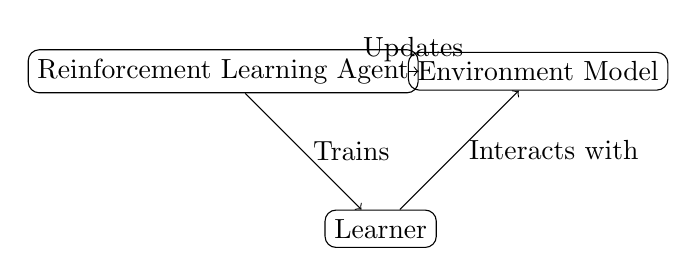
\begin{tikzpicture}
        % Nodes
        \node (agent) at (0, 0) [draw, rectangle, rounded corners] {Reinforcement Learning Agent};
        \node (env) at (4, 0) [draw, rectangle, rounded corners] {Environment Model};
        \node (learner) at (2, -2) [draw, rectangle, rounded corners] {Learner};
        
        % Arrows
        \draw[->] (agent) -- (learner) node[midway, right] {Trains};
        \draw[->] (learner) -- (env) node[midway, right] {Interacts with};
        \draw[->] (env) -- (agent) node[midway, above] {Updates};
        
    \end{tikzpicture}
    \caption{Diagram of the Distributed RL Framework}
    \label{fig:framework}
\end{figure}
